\chapter{Programming Arduino with C}
%------------------------------------------------
\par Arduino is it one of the most widely used micro-controller to develop various DIY projects. Developers design and assemble various sensors and other components to interact with environment. Being a controller, the board needs to be told and taught how, when, and where to communicate with other devices and environment. The process of instructing the controller what to do, step-by-step can be termed as programming. From being an art, programming is now an essential skill for any type of developer. To assist in developing various programs, developers have build various development tools to make programming easier and fun. 
\begin{marginfigure}
	\raggedright
    \vspace{-4cm}  
\includegraphics{Images/Programing_Arduino/IDE_startup.png}
\end{marginfigure}

\section{Programming the voltages}
\par A programming language is a set of grammatical rules that is understood by a device. At the basic level, all digital systems work by making a large number of voltage level switches. These voltage switches occur between two levels, high volt and a low volt (possibly zero volt). These large numbers of switching are represented by an array of bi (two) level patterns called binary language. This is what the machine understands, called the first generation language. It is very tedious and error-sum to program in binary language ( bunch of 1’s and 0’s ). Hence small English like mnemonics were used to program, forming the second generation language - assembly language. They are converted to a binary pattern using an assembler. To make development easier, more English like languages were developed like C, C++. They form the high level language - third generation language. They are converted to binary patterns using compilers and interpreters. There are fourth generation and fifth generation languages developed, meeting the demands of complex calculation. We would be tinkering around third generation language - C programming language to program Arduino Uno.

\section{Arduino IDE}


 \ac{IDE} contains necessary tools required to write, compile and upload our code (sketch) to Arduino. It is a open source, cross-platform application that is written in Java. It supplies a software library which provides many common input and output procedures. There are various form of Arduino \ac{IDE} - Arduino \ac{IDE} software (windwos, linux, mac systems), Arduino Web \ac{IDE} (runs on web browser), Arduinroid ( Andriod App ) that can be used to upload our sketch.

\begin{marginfigure}
	\raggedright
    \vspace{-4cm} 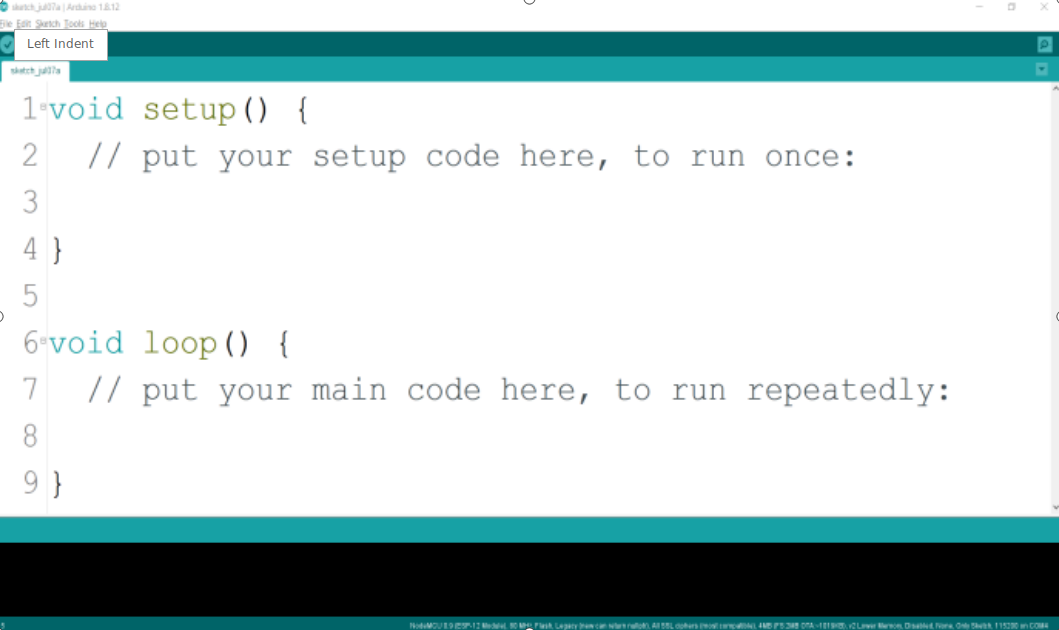
\includegraphics{Images/Programing_Arduino/IDE_interface.png}
    \captionsetup{type=figure}
    \caption{Arduino IDE}
\end{marginfigure}

\subsection{Parts of Arduino IDE}

\begin{enumerate}
    \item Verify : Checks the C program for errors
    \item Upload : Burns the compiled binary executable file into Arduino board
    \item New Tab : Open a new workspace to code
    \item Open : Opens new file
    \item Save : save current works
    \item Serial Monitor : Opens a new windows to conduct serial communications with the board
    \item Sketch : The current program that is been edited
    \item Code area : Areas to write code
    \item Message area : View message of boards
    \item Debug window : View status of boards
    \item Connection Info : View current connected board configurations
\end{enumerate}

\begin{marginfigure}
	\raggedright
    \vspace{-9cm} 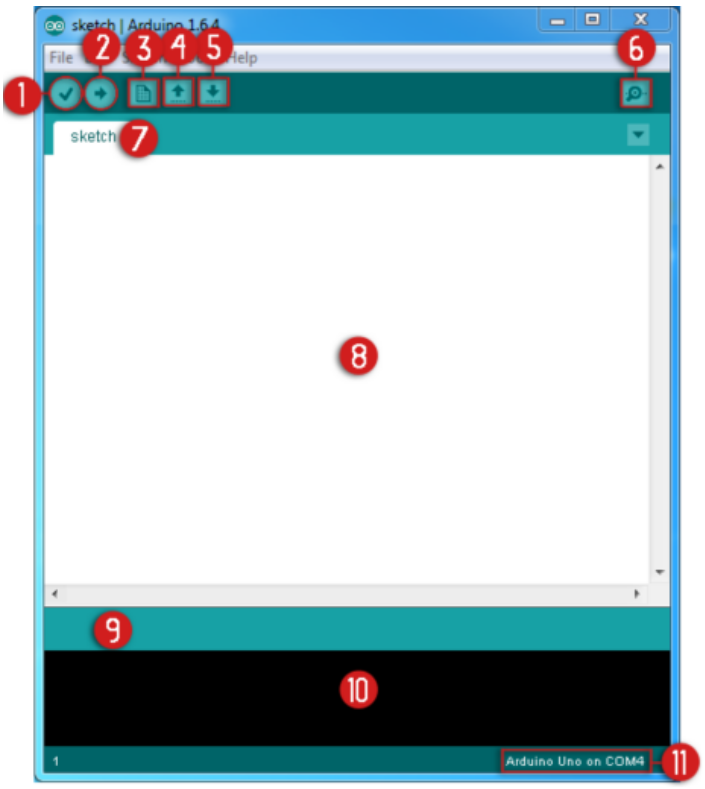
\includegraphics{Images/Programing_Arduino/ide_parts.png}
    \captionsetup{type=figure}
    \caption{Parts of \ac{IDE}}
\end{marginfigure}

\subsection{Arduino IDE : quick clicks}
\begin{enumerate}
    \item Install libraries\\
    They include code written by developers for certain sensors/usages.\\
    Tools -> Manage Libraries\\
    Shortcut : Ctrl + Shift + I
    
    \item Verify / compile\\
    Sketch -> Verify/Compile\\
    Shortcut : Ctrl + R
    
    \begin{marginfigure}
        \hspace{-4cm}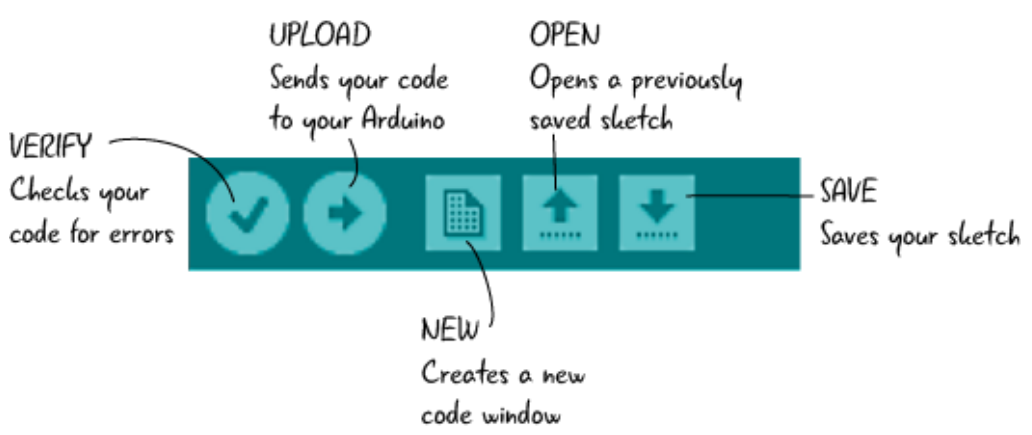
\includegraphics[width=3in]{Images/Programing_Arduino/quick_tool.png}
    \end{marginfigure}
    
    \item Upload\\
    Sketch -> Upload\\
    Shortcut : Ctrl + U
\end{enumerate}

\subsection{Steps to upload sketch to Arduino}
\begin{enumerate}
    \item Connect Arduino to PC
    \item Select board port from Tools -> Port
    \item Select board type from Tools -> Boards
    \item Save your code 
    \item Verify your code
    \item Upload your code
    \item Wait until code uploads. Watch the message box for status information.
\end{enumerate}

\section{Programming language for Arduino}
The official language for Arduino development is using the C/C++ programming language. C language is best known for its speed and close relationship with memory. C language can effectively make the most out of a given hardware optimally. The support for other programming languages is also being developed. Python language is gaining its support in Arduino. Take a look at \url{https://realpython.com/arduino-python/} to get started. Those who find difficulty in learning language, there are block codes available. It uses simple GUI to drag and drop various code block segments that are joined together to form a program. The automatically generated code can then be uploaded to Arduino. Take a look at \url{https://www.postscapes.com/iot-visual-programming-tools/} to get started. It would be best to write programs in C to get a clear understanding of the hardware and the program.

\begin{figure}
    \centering
    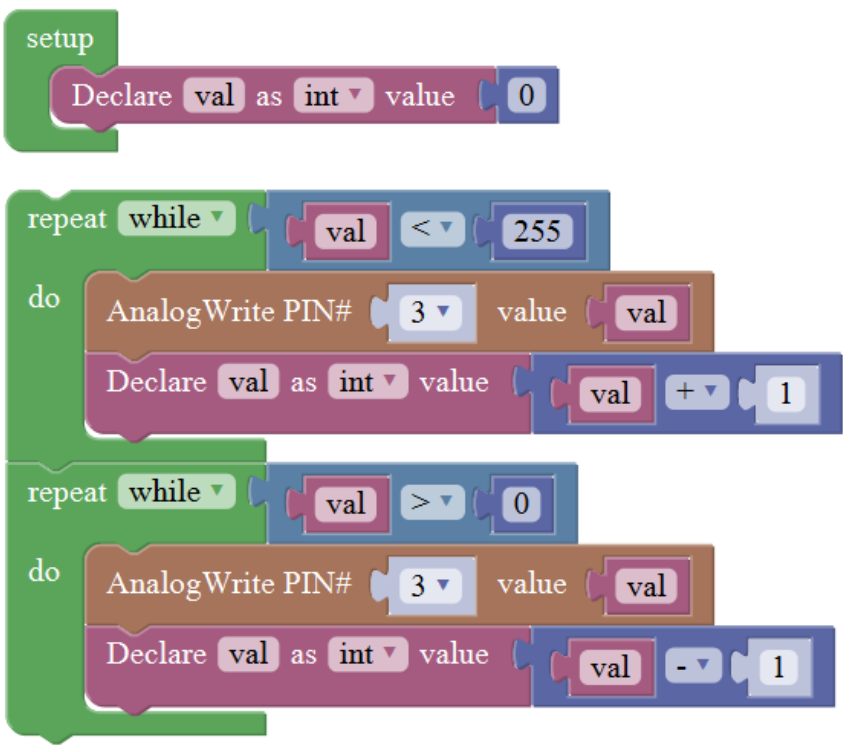
\includegraphics[width=2.8in]{Images/Programing_Arduino/block_code.png}
    \caption{block coding}
\end{figure}

\pagebreak
\section{Basic concepts of C language}
\begin{itemize}
    \item Data types \\
    Data types refers to the type of value we deal with. There are various types of data in C. They include characters, integers, decimal numbers etc. Each data occupy specific space in the memory to store and process those information Table \ref{tab:datatypes} shows few commonly used C data types and their memory consumption.
    
    
    \begin{table*}
        \renewcommand{\arraystretch}{1.5}
        \resizebox{\textwidth}{!}{%
            \begin{tabular}{|l|l|l|l|l|}
            \hline
            \multicolumn{1}{|c|}{\textit{\textbf{Data type}}} &
              \multicolumn{1}{c|}{\textit{\textbf{What value does it hold}}} &
              \multicolumn{1}{c|}{\textit{\textbf{Example}}} &
              \multicolumn{2}{c|}{\textit{\textbf{Memory Space}}} \\ \hline
            char        & Single characters                       & ‘a’, ‘b’, ‘Q’, ‘1’      & 1 byte  & 8 bit  \\ \hline
            int         & Integer numbers with no decimal parts   & -32768 to 32767         & 2 byte  & 16 bit \\ \hline
            long int    & Same as int type, with longer precision & 2147483, 647885425      & 4 byte  & 32 bit \\ \hline
            float       & Number with decimal point               & 2.312, 2.2258 etc       & 4 byte  & 32 bit \\ \hline
            double      & Same as float, with longer precision    & 2.59874, 69.88524589    & 8 byte  & 64 bit \\ \hline
            long double & Same as double, with longer precision   & 658.8885421, 9986.22104 & 10 byte & 80 bit \\ \hline
        \end{tabular}%
        }
        \vspace{3mm}
        \caption{Datatypes in C}
        \label{tab:datatypes}
    \end{table*}
    
    \item Variables \\
    Data are stored in specific memory location. These memory location names are difficult to handle. Hence we name those locations for easy access. These names are called as variables. They simply refers to a named storage location in the memory.\\
    General syntax : 
    \begin{lstlisting}[style=CStyle]
        <data type> <variable name>;
    \end{lstlisting}
    Example
    \begin{lstlisting}[style=CStyle]
        int number = 5;
        float pie = 3.14;
    \end{lstlisting}
    
    \item Statements \\
    It refers to an instruction that instructs to do a specific task. In C language, statements are ended with semicolon( ; ) There are different types of statements. Some of them are conditional statement, iteration statements, jump statements.
    
    \item Functions \\
    They refers to a group/set of instructions referenced under one name. They increase program readability and is easy to extend a feature or find errors. We can pass value to a function - called parameters. We are free to define our own functions. However, certain functions are defined by the system and are reserved.
    
    \item Conditional statements \\
    These statements directs the control of the program execution based on some conditions.\\
    General syntax:
    \begin{lstlisting}[style=CStyle]
        if( condition ) 
        {
            Statements to execute if condition is true
        }
        else
        {
            Statements to execute if condition is false
        }
    \end{lstlisting}
    
    \item Looping statements \\
    These statements executes a set of statements until some condition holds true. There are three types of loops, namely - for loops, while loops and do while loops \\
    General syntax - for loop :
    \begin{lstlisting}[style=CStyle]
        for(initialization ; condition ; updation) 
        {
            Statements to be executed
        }
    \end{lstlisting}
    General syntax - while loop:
    \begin{lstlisting}[style=CStyle]
        while( condition ) 
        {
            Statements to be executed
        }
    \end{lstlisting}
    General syntax - do while loop:
    \begin{lstlisting}[style=CStyle]
    do{
        Statements to be executed
    }while (condition);
    \end{lstlisting}

    
    \item Arithmetic - Comparison - Logical operators\\
    Operators gives us the power to manipulate various data. Table \ref{tab:arithmetic} shows the available operators that can be used with numbers. Table \ref{tab:comparision} shows various comparison operators that can be used make decisions. At times, we would require more than one conditions to be satisfied. Table \ref{tab:logical} show how we can club different conditions to create single decision.
    
    \begin{table}
        \centering
        \renewcommand{\arraystretch}{1.5}
        \begin{tabular}{|c|l|}
            \hline
            \textit{\textbf{Symbol}} & \multicolumn{1}{c|}{\textit{\textbf{Meaning}}}   \\ \hline
            +                        & Addition                                         \\ \hline
            -                        & Subtraction                                      \\ \hline
            /                        & Division                                         \\ \hline
            *                        & Multiplication                                   \\ \hline
            \%                       & Modulus -\textgreater returns the remainder      \\ \hline
            ++                       & Unary addition -\textgreater adds by one         \\ \hline
            --                       & Unary subtraction -\textgreater subtracts by one \\ \hline
        \end{tabular}
        \caption{Arithmetic Operators}
        \label{tab:arithmetic}
    \end{table}
    
    \begin{table}
        \centering
        \renewcommand{\arraystretch}{1.5}
        \begin{tabular}{|c|c|}
        \hline
            \textit{\textbf{Symbol}} & \textit{\textbf{Meaning}} \\ \hline
            > & Greater than \\ \hline
            < & Less than \\ \hline
            >= & Greater than or equal to \\ \hline
            <= & Less than or equal to \\ \hline
            == & Both are equal? \\ \hline
        \end{tabular}
        \caption{Comparison Operators}
        \label{tab:comparision}
    \end{table}
    
    \begin{table*}
        \renewcommand{\arraystretch}{1.5}
        \begin{tabular}{|c|c|l|}
            \hline
            \textit{\textbf{Symbol}}                                                 & \textit{\textbf{Name}} & \multicolumn{1}{c|}{\textit{\textbf{Meaning}}} \\ \hline
            \textless{}condition\textgreater \&\& \textless{}condition\textgreater{} & AND                    & True if both conditions are True               \\ \hline
            \textless{}condition\textgreater || \textless{}condition\textgreater{}   & OR                     & True if any of the conditions are True         \\ \hline
            ! \textless{}condition\textgreater{} & NOT & True if condition is false \\ \hline
        \end{tabular}
        \vspace{3mm}
        \caption{Logical Operators}
        \label{tab:logical}
    \end{table*}

\end{itemize}

\subsection{Arduino specific functions and usages}
\par Arduino have a bunch of functions that are used by the Arduino board for its functioning. Below are few of the commonly used functions. Additional function and their usages can be found at \url{https://www.arduino.cc/reference/en/}

\begin{itemize}
    \item void setup()\\
    This is an unavoidable function. The statements written in this function are executed exactly once. Whenever Arduino starts ( or reset button is pressed) the program execution starts from this function. Usually the declaration part and other configuration are written here, that needs to be executed only once. After its execution, it automatically calls the void loop() function.
    
    \item void loop()\\
    This is an unavoidable function. The statements written in this function are executed again and again. This part consist of the core part of the program. Statements like monitoring a sensor, reading pins etc are written here. The Arduino never stops its execution. On reaching the end of loop(), it would execute the same function again.
    
    \item pinMode() \\
    This function determines how the pins of the board needs to be interfaced. It configures general purpose input output pins as input mode or output mode. Prior to using the pin, every pin must have its mode defined using this function. It is usually written in void setup() function.\\
    General syntax:
    \begin{lstlisting}[style=CStyle]
        pinMode(<pin number>, INPUT | OUTPUT | INPUT_PULLUP );
    \end{lstlisting}
    Example:
    \begin{lstlisting}[style=CStyle]
        //pin 13 is configured as output mode
        pinMode(13, OUTPUT);  
    \end{lstlisting}
    
    \item Serial monitor\\
    Serial monitor is a window that can be found in Arduino \ac{IDE}, that facilitates serial communication with Arduino. Streams of data can flow from the monitor to Arduino and from Arduino to the system. For Arduino to listen for serial communication, Serial service must be initiated at a specific baud rate. Baud rate is the rate at which Arduino speaks to the system. Usually 9600 bits per second is set as the baud rate.\\ 
    Example : Printing to Serial monitor
    \begin{lstlisting}[style=CStyle]
    int value = 55;
    
    void setup(){
        //starting serial communication
        Serial.begin(9600);
            
        //Print a line to monitor and go to new line
        Serial.println("Device started");
        
        //Print a line to monitor and remain in same line
        Serial.print("value = ");

        //Print a data inside a variable
        Serial.println(value);
    }
    void loop(){
        //do nothing
    }
    \end{lstlisting}
    
    \item digitalRead() \\
    This function is used to read the digital state of a pin configured as INPUT mode. If the pin have a voltage above 2.5V, the function returns HIGH ( = 1). If the pin have a voltage below 2.3V, the function returns LOW ( = 0).\\
    General syntax:
    \begin{lstlisting}[style=CStyle]
        state = digitalRead(<pin number>);
    \end{lstlisting}
    Example:
    \begin{lstlisting}[style=CStyle]
        //reads status of INPUT pin 12
        int state = digitalRead(12);  
    \end{lstlisting}
    
    \item digitalWrite()\\
    This function is used to set the voltage of an OUPUT mode pin to 5V or 0V. If the pin is set to HIGH, we would get 5V at the pin. If the pin is set to LOW, we would get 0V at the pin.\\
    General syntax:
    \begin{lstlisting}[style=CStyle]
        digitalWrite(<pin number>, HIGH | LOW);
    \end{lstlisting}
    Example:
    \begin{lstlisting}[style=CStyle]
        //turn on in-build LED of Arduino Uno : set to 5V
        digitalWrite(13,HIGH);
        
        //sets the voltage level to 0V
        digitalWrite(12,LOW);     
    \end{lstlisting}
    
    \item analogRead()\\
    This function is used to read the analog values analog pin configured as INPUT mode. Analog pin varies from A0 to A5. The analog to digital converter (ADC) maps the voltage at the input pin into a 10 bit number. Table \ref{tab:analog_in_mapping} summarizes the voltage to value mapping of the function.
    
    \begin{table}
        \centering
        \begin{tabular}{|c|c|}
            \hline
            \multicolumn{1}{|l|}{\textit{\textbf{Voltage at analog input pin}}} & \multicolumn{1}{l|}{\textit{\textbf{10bit value returned}}} \\ \hline
            0V   & 0    \\ \hline
            1V   & 205  \\ \hline
            2.5V & 512  \\ \hline
            5V   & 1023 \\ \hline
        \end{tabular}
        \caption{Analog to Digital mapping}
        \label{tab:analog_in_mapping}
    \end{table}
    \vspace{3mm}
    General syntax:
     \begin{lstlisting}[style=CStyle]
        value = analogRead(<pin number>);
    \end{lstlisting}
    Example:
     \begin{lstlisting}[style=CStyle]
        //read 10bit mapped voltage of A2 analog input pin
        int state = analogRead(A2);  
    \end{lstlisting}

    \item analogWrite()\\
    This function is used to produce analog output values at the \ac{PWM} pins configured as OUTPUT mode. \ac{PWM} supported pins in Arduino Uno are 3, 5, 6, 9, 10, 11. The \ac{PWM} technique maps the 8bit numbers to 5V voltage output. Table \ref{tab:analog_out_mapping} summarizes the functions.
    
    \begin{table}
        \centering
        \begin{tabular}{|c|c|c|}
            \hline
            \textit{\textbf{Value passed}} & \textit{\textbf{Duty cycle}} & \textit{\textbf{Voltage experienced}} \\ \hline
            0   & 0 \%    & 0V    \\ \hline
            50  & 19.92\% & 0.99V \\ \hline
            127 & 50\%    & 2.5V  \\ \hline
            255 & 100\%   & 5V    \\ \hline
        \end{tabular}
        \caption{Digital to Analog Mapping}
        \label{tab:analog_out_mapping}
    \end{table}
    \vspace{3mm}
    
    General syntax:
     \begin{lstlisting}[style=CStyle]
        analogWrite(<pin number>, <8bit number>);
    \end{lstlisting}
    Example:
     \begin{lstlisting}[style=CStyle]
        //Set the voltage at pin 5 as 2.5V
        analogWrite(5,127);  
    \end{lstlisting}
    
    \item delay()\\
    This function is used pause the execution of program for a defined time. It accepts an integer denoting the number of milliseconds to be paused.\\
    General syntax:
     \begin{lstlisting}[style=CStyle]
        delay(<milliseconds>);
    \end{lstlisting}
    Example:
     \begin{lstlisting}[style=CStyle]
        delay(1000);  //pauses for 1 second
    \end{lstlisting}
        
    \item delayMicroseconds()\\
    This function is used pause the execution of program for a defined time. It accepts an integer denoting the number of microseconds to be paused.\\
    General syntax:
    \begin{lstlisting}[style=CStyle]
        delayMicroseconds(<microseconds>);
    \end{lstlisting}
    Example:
     \begin{lstlisting}[style=CStyle]
        delayMicroseconds(10);  //pauses for 10 microsecond
    \end{lstlisting}
\end{itemize}

\vspace{1cm}

There are a lot of additional functions defined for Arduino Development. Furthermore, developers around the world have contributed various additional methods to facilitate easy development. These works are compiled into small library, whose codes are made public. These libraries can be easily downloaded and made available via library manager in Arduino \ac{IDE}. Additional methods are also written for various types of Arduino boards. 

\newpage
\section{Example Programs}
    \subsection{Blinking an LED}
    \begin{lstlisting}[style=CStyle]
    int LED=13;
    
    void setup(){
        pinMode(LED,OUTPUT);		
        Serial.begin(9600);
    }
    
    void loop(){
        digitalWrite(LED,HIGH);
        Serial.println("LED turned ON");
        delay(1000);
    
        digitalWrite(LED,LOW);
        Serial.println("LED turned OFF");
        delay(1000);
    }
    \end{lstlisting}
    \begin{figure}
        \centering
        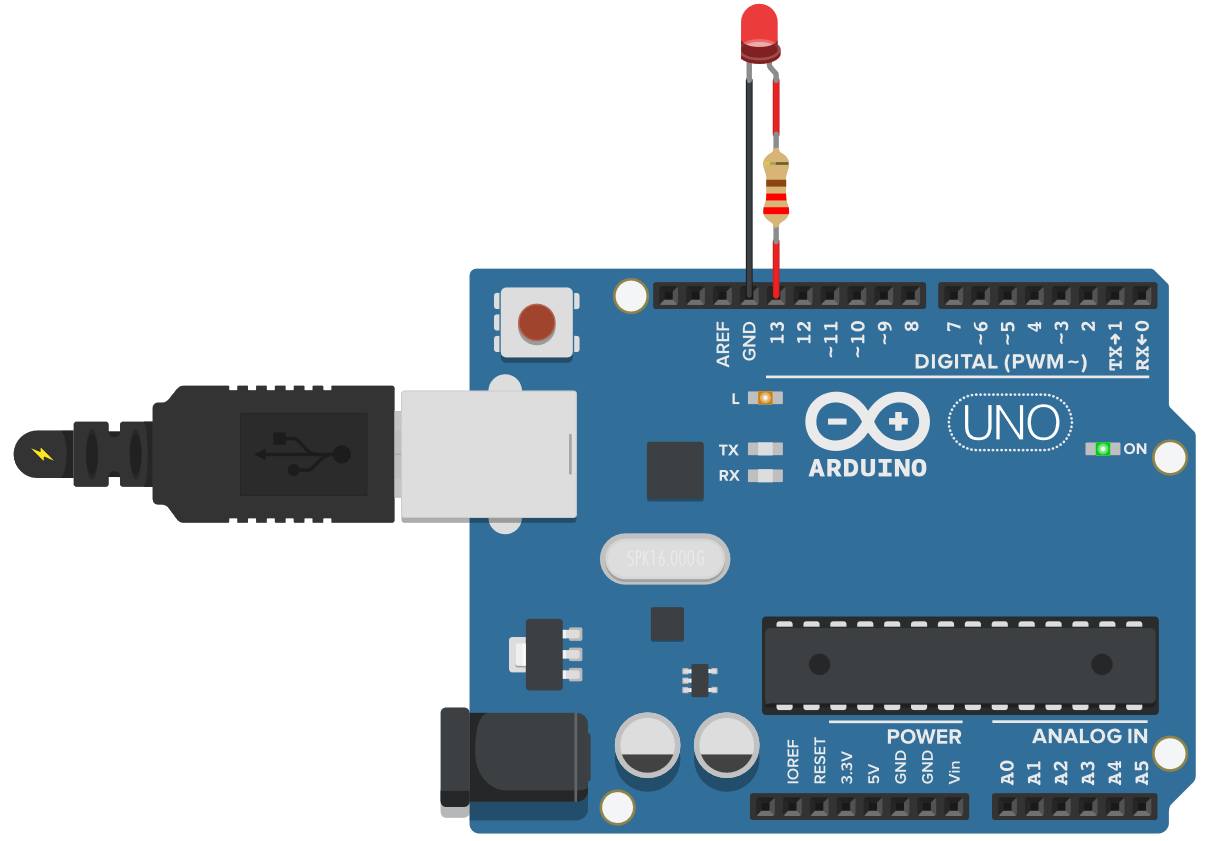
\includegraphics{Images/Programing_Arduino/led_blink_ckt.png}
        \caption{Led Blinking circuit}
    \end{figure}

    \newpage
    \subsection{Interfacing Push Button}
    \par Buttons physically isolates the circuit. The circuit is closed only when the button is pressed. When the button is not pressed, the INPUT pin associated with that button feels that nothing is connected and in-circuit effects can affect the voltage. If the voltage falls below 2.3V, we will read low signal. If the voltage falls above 2.5V, we will read high signal. If the voltage stands between 2.3V and 2.5V, we cannot predict the output. 
    
    \begin{marginfigure}
        \centering
        \subfloat[Pullup config]{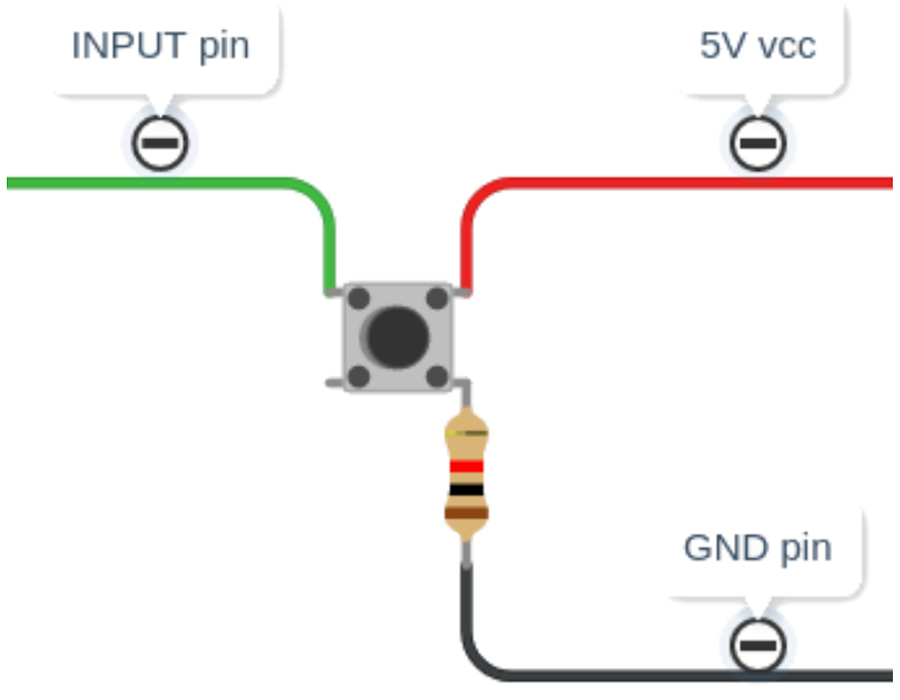
\includegraphics[width=1.5in]{Images/Programing_Arduino/pullup_config.png}}\\
        \subfloat[Pulldown config]{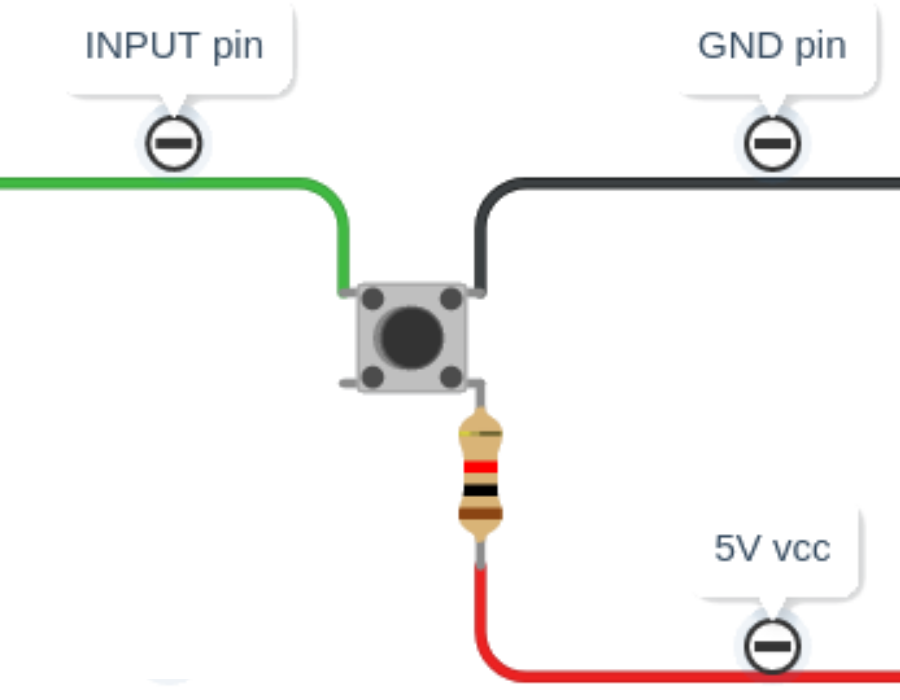
\includegraphics[width=1.5in]{Images/Programing_Arduino/pulldown_config.png}}
        \captionsetup{type=figure}
        \caption{Button configuration}
        \label{fig:button_config}
    \end{marginfigure}
    
    Hence push buttons are interfaced by building pullup circuits or pulldown circuit configuration as shown in figure \ref{fig:button_config} . In pullup configuration, if the button is not pressed, the 5V is connected to the pin. When the button is pressed, the pin will be connected to the ground (0V). The opposite happens in pulldown configuration. However, instead of building these circuits, we can implement the pullup circuit via the small internal resistor of the board. To avail such capability, we need to declare the pin as \textbf{INPUT\_PULLUP} mode.

    \begin{lstlisting}[style=CStyle]
    int button = 12;
    int state;

    void setup(){
        pinMode(button,INPUT_PULLUP);
        Serial.begin(9600);
        }
    void loop(){
        state = digitalRead(button);
        if( state == LOW ){
            Serial.println("Button pressed");
        }
        else{
            Serial.println("Button not pressed");
        }
        delay(500);
    }
    \end{lstlisting}
    
    \begin{figure}
        \centering
        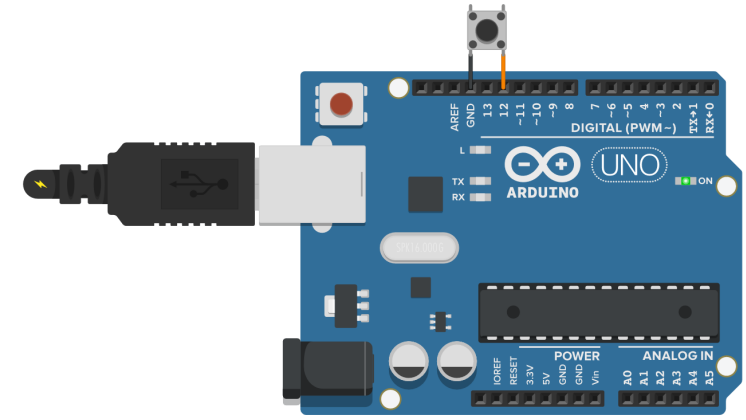
\includegraphics[width=4.2in]{Images/Programing_Arduino/button_ckt.png}
        \caption{Push button circuit}
    \end{figure}
    
    \newpage
    \subsection{Reading analog values : Interfacing potentiometer}
    \begin{lstlisting}[style=CStyle]
    int pot_pin = A0;
    
    void setup(){
        pinMode(pot_pin, INPUT);
        Serial.begin(9600);
    }
    
    void loop(){
        int range = analogRead(pot_pin);
        Serial.print("Analog value: ");
        Serial.println(range);
    }
    \end{lstlisting}
    
    \begin{figure}
        \centering
        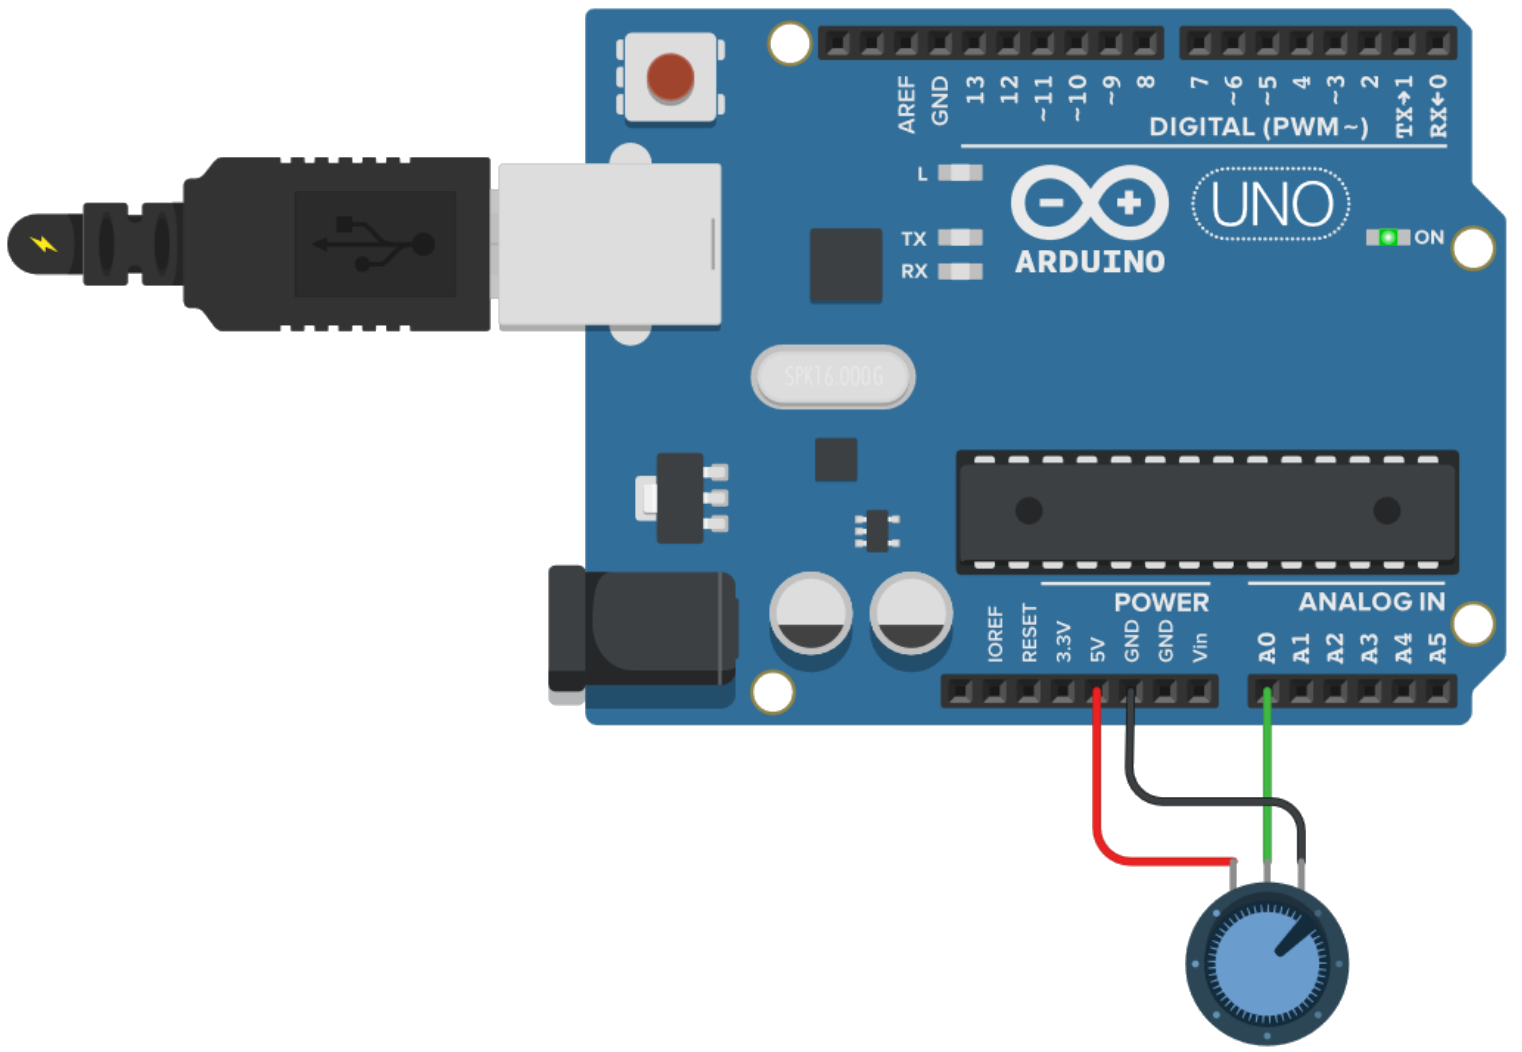
\includegraphics{Images/Programing_Arduino/potentio_ckt.png}
        \caption{Potentiometer circuit}
    \end{figure}

    \newpage
    \subsection{Writing analog values : Fading LED}
    \begin{lstlisting}[style=CStyle]
    int LED=11;
    int bright;
    
    void setup(){
        pinMode(LED,OUTPUT);		
        Serial.begin(9600);
    }
    
    void loop(){
        Serial.println("Turning ON");
        for(bright = 0; bright<= 255; bright++){
            analogWrite(LED,bright);
            delay(500);
        }
        
        Serial.println("Turning OFF");
        for(bright = 255; bright>= 0; bright--){
            analogWrite(LED,bright);
            delay(500);
        }
    }
    \end{lstlisting}

    \begin{figure}
        \centering
        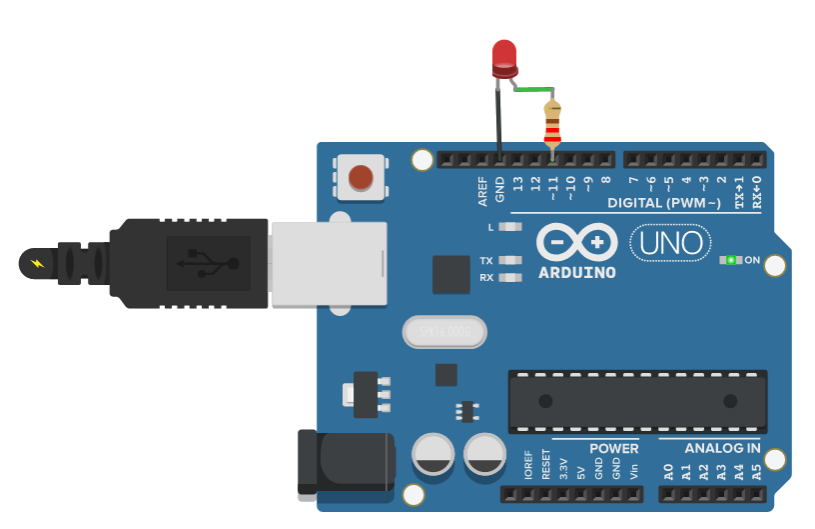
\includegraphics{Images/Programing_Arduino/fading_ckt.png}
        \caption{LED fading circuit}
    \end{figure}














